\chapter{Reviews}
\label{vl:tc-review}

\dword{jpo} and \dword{tc} review all stages of detector development
and work with each consortium to arrange reviews of the design
(\dword{cdrev}, \dword{pdr} and \dword{fdr}), production (\dword{prr}
and \dword{ppr}), installation (\dword{irr}) and operation
(\dword{orr}) of their system.  These reviews provide information to
the \dword{tb} and \dword{exb} to help in evaluating technical
decisions. A timeline for the review process is shown in
Figure~\ref{fig:review_timeline}.
\begin{dunefigure}[DUNE review process]{fig:review_timeline}
  {\dword{dune} review process and timeline}
  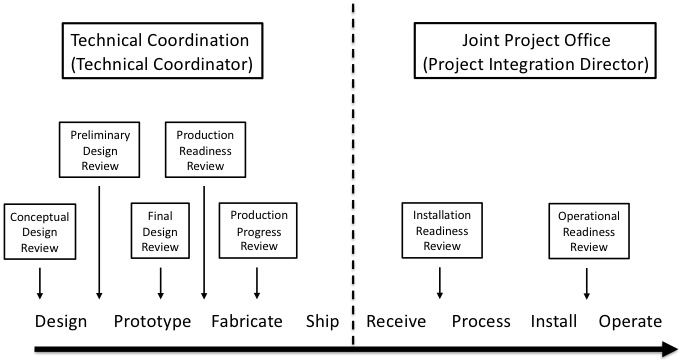
\includegraphics[width=0.75\textwidth]{review_timeline}
\end{dunefigure}
Review reports are tracked by \dword{jpo} and \dword{tc} and provide
guidance on key issues that require engineering oversight by the
\dword{tc} engineering team. \dword{tc} maintains a calendar of
\dword{dune} reviews.

\dword{tc} works with consortia leaders to review all detector
designs.  As part of the \dword{tdr} development \dwords{pdr} are
planned for subsystems in advance of the \dword{tdr} followed by
\dwords{fdr} after the \dword{tdr}.  All major technology decisions
will be reviewed before down-select.  \dword{tc} may form task forces
as needed to address specific issues that require more in depth
review.


Production of detector elements begins only after successful
\dwords{prr}. Regular production progress reviews will be held once
production starts. The \dwords{prr} will typically include a review of
the production of \textit{Module 0}, the first module produced at the
facility. \dword{tc} will work with consortia leaders on all
production reviews.

\dword{tc} coordinates technical documents for the \dword{lbnc}
\dword{tdr} review.

The review process is an important part of the \dword{dune} \dword{qa}
process as described in Section~\ref{sec:verification}, for
design and production.

The review process has been in place since 2016 with various reviews
of \dword{protodune} components and has continued into the first
\dword{dune} reviews in 2018--19. Past and scheduled reviews are in
the \dword{dune} Indico at https://indico.fnal.gov/category/586.
Review reports are in DocDB-1584.

\section{Design Reviews}

The \dword{dune} design review process is described in DocDB-9664 and
is consistent with the \fnal review process described in
http://eshq.fnal.gov/manuals/feshm. Design reviews for
\dword{protodune} were held for each major system. Because the
schedule was extremely tight for \dword{protodune}, only a single
design review was held for each system.

The successful operation of \dword{protodune} means \dword{dune} is at
a very advanced state of design. The strategy going forward is to hold
\dword{cdrev} for systems with significant changes from
\dword{protodune}. These systems include the \dword{dss}, \dword{pds},
\dword{daq} and calibration. All systems will go through \dwords{pdr}
to review design changes from \dword{protodune} and \dwords{fdr} after
the \dword{tdr}.

\dword{tc} has established an Engineering Safety Committee with
mechanical and electrical engineering experts from collaborating
institutions to develop processes and procedures to evaluate
engineering designs using accepted international safety standards. The
current status of international code equivalencies is discussed
further in Section~\ref{sec:esh_codes}. The codes and standards to
which each system is designed will be reviewed as part of the
\dword{pdr} and \dword{fdr}.

\section{Production Reviews}

Once the designs are finished, production reviews will be held before
significant funds are authorized for large production runs. These
reviews are closely coordinated with the \dword{qa} team. The
expectation is that a \textit{Module 0} be produced and presented as
part of the \dword{prr}.

Once production has started, \dword{tc} will schedule \dwords{ppr}
as appropriate to monitor production schedule and quality.

\section{Installation Reviews}

\dwords{irr} are planned to verify equipment and procedures are in
place prior to installation of the detector components. A critical
part of these reviews is to establish and verify the \dword{ha} for
the installation activities and mitigate any safety risks.

\section{Operations Reviews}

\dwords{orr} (http://eshq.fnal.gov/manuals/feshm/\#series2000) are the
final safety check out before equipment can be operated.

\section{Review Tracking}

Tracking and controling review recommendations is part of the review
process. Review committees assess recommendations from earlier
reviews. \dword{tc} assures that the consortia respond to review
recommendations and works with the consortia to make sure the
responses are appropriately documented and implemented. Reports from
\dword{dune} reviews are maintained in DocDB-1584 along with the list
of recommendations.


%%%%%%%%%%%%%%%%%%%%%%%%%%%%%%%%
\section{Lessons Learned}
\label{sec:fdsp-coord-lessons}

A detailed list of lessons learned from construction and operation of
\dword{pdsp} is in~\cite{bib:docdb8255}. These lessons have driven planning for
\dword{dune} and have led to design changes in \dword{dune}. Lessons
learned will continue to be updated throughout design review process
and into production. The methodologies are described in
Section~\ref{sec:quality_improvement}. %{sec:lessons_learned}.


%%%%%%%%%%%%%%%%%%%%%%%%%%%%%%%%
\section{Reporting}
\label{sec:fdsp-coord-reporting}

The \dword{dune} project has published regular monthly reports since
the final design and construction of \dword{protodune} began in
earnest in summer 2016. \dword{tc} will continue to compile and
publish these reports. Reporting will expand to include monthly
reports against the \dword{ims}. The \dword{dune} project provides
regular reports to the \dword{lbnc} at reviews several times a
year. The \dword{dune} project produces reports from design,
production and operations reviews.
